\chapter{Cơ sở lý thuyết}
% =======================
% PHẦN 1: LÝ THUYẾT VỀ PLC VÀ HMI
% =======================
\section{PLC Mitsubishi và HMI PFXGP4501TAA}

\subsection{PLC Mitsubishi Q13UDVCPU}

Bộ điều khiển logic khả trình (PLC) Mitsubishi Q13UDVCPU (Hình \ref{c2:plc_q13udvcpu}) thuộc dòng MELSEC-Q Series, là CPU đa năng có hiệu suất xử lý cao và khả năng mở rộng linh hoạt. Với tốc độ thực thi lệnh cơ bản 1,9~ns, dung lượng chương trình 130K~steps và khả năng quản lý tới 8.192 điểm I/O, Q13UDVCPU đáp ứng tốt các yêu cầu của các dây chuyền sản xuất hiện đại, nơi cần xử lý nhanh, ổn định và có độ tin cậy cao \cite{mitsubishi_q13udvcpu}.

CPU tích hợp sẵn các giao tiếp Ethernet, USB và khe cắm thẻ SD, cho phép kết nối thuận tiện với thiết bị ngoại vi, mạng công nghiệp hoặc hệ thống SCADA. Nhờ khả năng mở rộng mạnh mẽ, Q13UDVCPU được sử dụng rộng rãi trong tự động hóa công nghiệp, đặc biệt khi kết hợp với HMI để giám sát và vận hành hệ thống.

\begin{figure}[h]
    \centering
    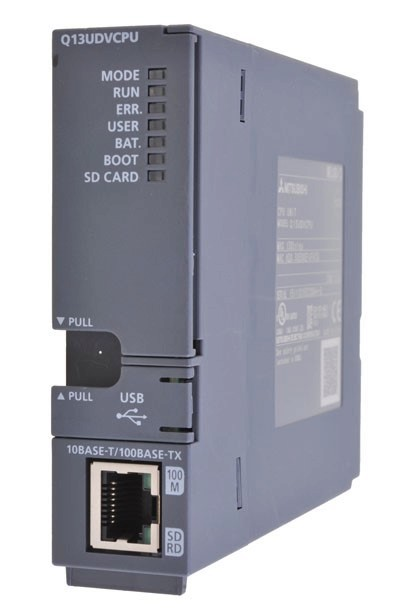
\includegraphics[width=0.33\textwidth]{figures/Chapter2/plc-cpu.png}
    \caption{CPU Mitsubishi Q13UDVCPU}
    \label{c2:plc_q13udvcpu}
\end{figure}

Một hệ thống PLC Mitsubishi Q Series cơ bản (Hình \ref{c2:plc-structure}) bao gồm các thành phần: module nguồn (Power Supply), khung base unit, CPU Q13UDVCPU và các module mở rộng I/O hoặc truyền thông. Module nguồn được lắp tại vị trí ngoài cùng bên trái nhằm cấp điện cho toàn bộ rack. CPU Q13UDVCPU được gắn trực tiếp lên base unit, tiếp theo là các module mở rộng như I/O số, I/O tương tự, module truyền thông (ví dụ CC-Link) hoặc module điều khiển chuyển động (motion).

Việc lắp đặt cần đảm bảo các đầu nối tiếp xúc chắc chắn, hạn chế bụi bẩn và rung động để đảm bảo độ ổn định của hệ thống. Sau khi hoàn tất phần cứng, PLC được cấu hình trên phần mềm GX Works2 hoặc GX Developer. Quá trình cấu hình bao gồm khai báo CPU, module nguồn, các module I/O đúng theo vị trí lắp thực tế. Nếu hệ thống sử dụng remote rack, địa chỉ truyền thông cũng cần được thiết lập tương ứng. Cấu hình chính xác giúp hệ thống hoạt động ổn định và tránh lỗi khi chạy chương trình điều khiển.

\begin{figure}[h]
    \centering
    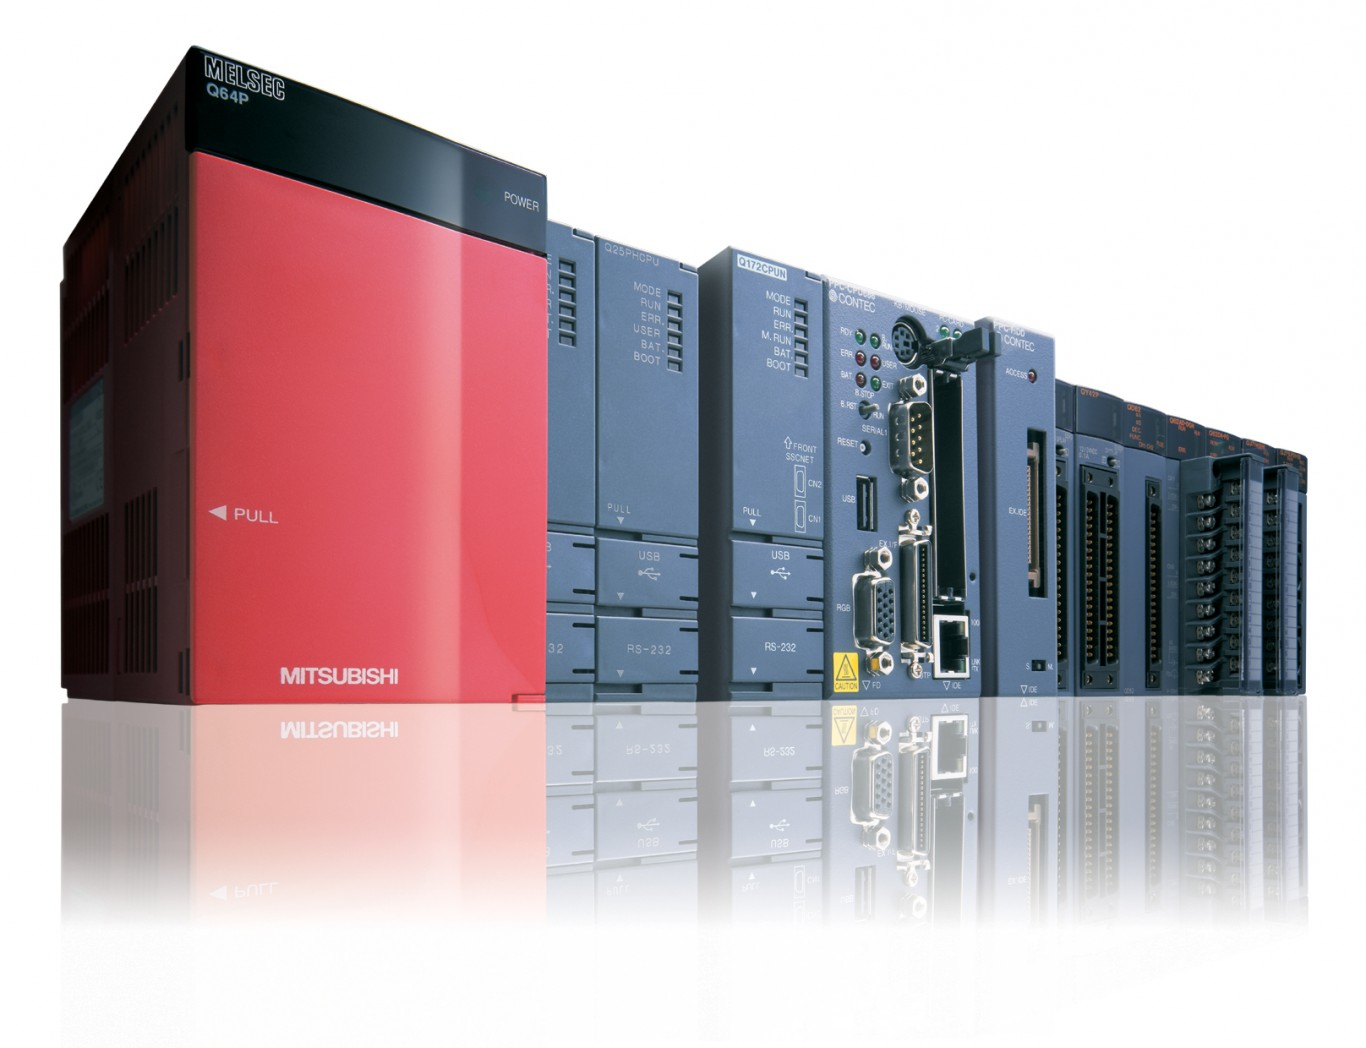
\includegraphics[width=0.75\linewidth]{figures/Chapter2/plc-structure.png}
    \caption{Hệ thống PLC Mitsubishi Q Series}
    \label{c2:plc-structure}
\end{figure}
\begin{table}[h]
\centering
\caption{Thông số kỹ thuật của PLC Mitsubishi Q13UDVCPU}
\label{tab:q13udvcpu_specs}
\begin{tabularx}{\textwidth}{|X|X|}
\hline
\textbf{Thông số} & \textbf{Giá trị} \\ \hline
Tốc độ xử lý lệnh (LD) & 1,9 ns \\ \hline
Dung lượng chương trình & 130K steps (520 kB) \\ \hline
Bộ nhớ RAM tích hợp & 1.024 kB \\ \hline
Thẻ nhớ hỗ trợ & SD/SDHC tối đa 32 GB \\ \hline
I/O tối đa (cục bộ) & 4.096 điểm \\ \hline
I/O tối đa (toàn hệ thống) & 8.192 điểm \\ \hline
Giao tiếp tích hợp & Ethernet 10/100 Mbps, USB \\ \hline
Nguồn tiêu thụ nội bộ & 0,58 A \\ \hline
Kích thước & 98 × 27,4 × 115 mm \\ \hline
Khối lượng & 0,20 kg \\ \hline
Nhiệt độ làm việc & 0 … 55 °C \\ \hline
Độ ẩm làm việc & 5 … 95\% RH (không ngưng tụ) \\ \hline
Chuẩn chống rung/sốc & JIS B 3502, IEC 61131-2 \\ \hline
\end{tabularx}
\end{table}

Phần mềm lập trình và cấu hình phổ biến cho PLC Mitsubishi Q13UDVCPU là GX Works2 \cite{gxworks2_simpleproject_manual}. Đây là môi trường phát triển tích hợp (IDE) hỗ trợ các ngôn ngữ lập trình IEC~61131-3 như Ladder Diagram (LD), Structured Text (ST) và Function Block Diagram (FBD)\cite{mitsubishi_plc_ladder_manual}. Trong GX Works2, người dùng tiến hành khai báo CPU, module nguồn, module I/O, module truyền thông hoặc motion theo đúng vị trí vật lý trên base unit. Phần mềm cũng hỗ trợ thiết lập tham số mạng (Ethernet, CC-Link), quản lý bộ nhớ, tải/chỉnh sửa chương trình qua USB hoặc Ethernet, và chức năng giám sát trạng thái online theo thời gian thực, hỗ trợ hiệu quả cho quá trình kiểm tra và gỡ lỗi.

\subsection{Giao diện người–máy HMI PFXGP4501TAA}

Giao diện Người–Máy (Human–Machine Interface, HMI) là thiết bị cho phép người vận hành tương tác trực tiếp với hệ thống điều khiển thông qua màn hình trực quan. Trong hệ thống này, HMI đảm nhiệm vai trò giám sát trạng thái, hiển thị dữ liệu sản xuất, cảnh báo lỗi và nhận lệnh vận hành từ người dùng, giúp đơn giản hóa quá trình điều khiển và giảm thiểu sai sót.

Màn hình HMI PFXGP4501TAA thuộc dòng GP4000 Series của hãng Pro-face (Schneider Electric), là thiết bị giao diện phổ biến nhờ thiết kế chắc chắn, độ ổn định cao và khả năng kết nối tốt với PLC Mitsubishi Q Series (Hình \ref{c2:hmi}).

Thiết bị được cấu hình bằng phần mềm GP-Pro EX, cho phép thiết kế giao diện, thiết lập truyền thông với PLC và xây dựng các màn hình giám sát một cách linh hoạt. Nhờ hỗ trợ nhiều giao thức công nghiệp và khả năng trực quan hóa dữ liệu tốt, HMI PFXGP4501TAA đóng vai trò quan trọng trong việc nâng cao hiệu quả vận hành và giám sát dây chuyền tự động hóa.

\begin{figure}[h]
    \centering
    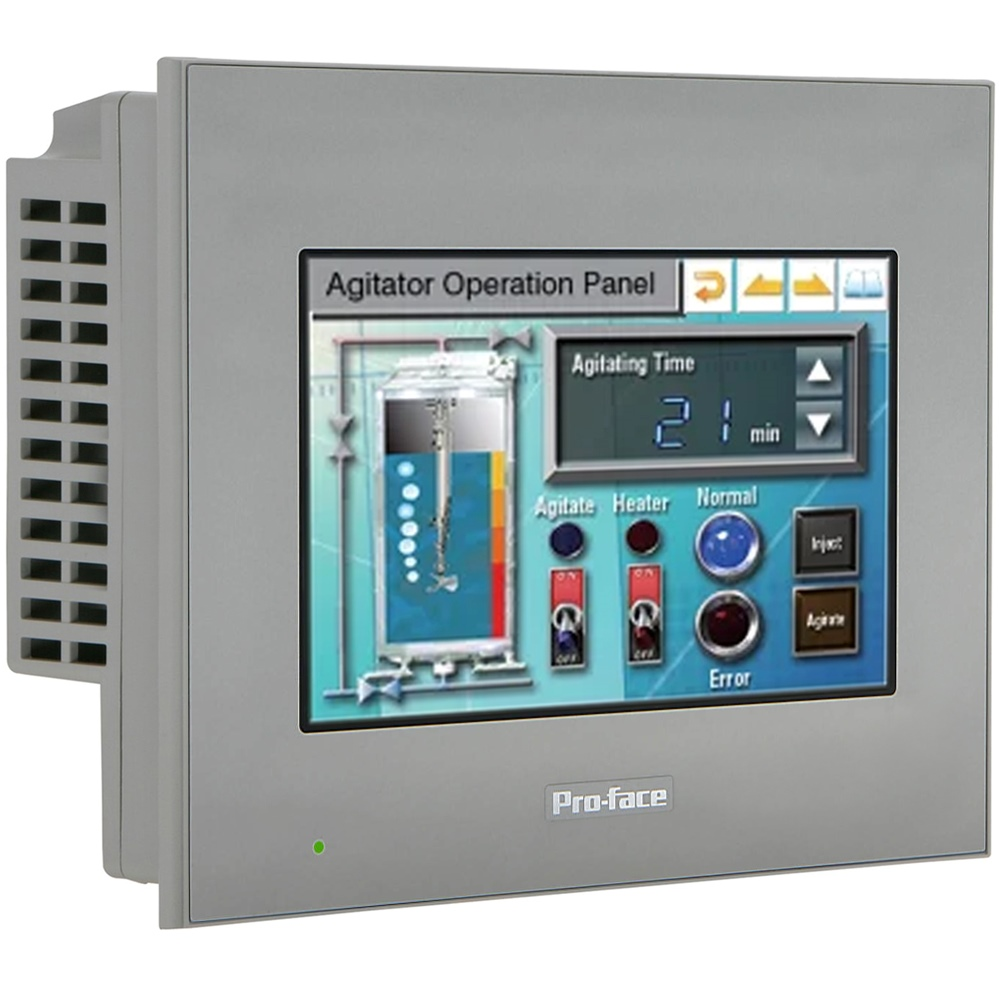
\includegraphics[width=0.43\textwidth]{figures/Chapter2/pfxgp4501taa.jpg}
    \caption{Màn hình HMI Pro-face PFXGP4501TAA}
    \label{c2:hmi}
\end{figure}

\begin{table}[h]
\centering
\caption{Thông số kỹ thuật của HMI PFXGP4501TAA}
\label{tab:hmi_specs}
\begin{tabular}{|l|l|}
\hline
\textbf{Thông số} & \textbf{Giá trị} \\ \hline
Kích thước màn hình & 10,4 inch TFT LCD \\ \hline
Độ phân giải & 640 × 480 (VGA) \\ \hline
Màu hiển thị & 65.536 màu \\ \hline
Độ sáng & 300 cd/m\textsuperscript{2} \\ \hline
Cổng giao tiếp & Ethernet, USB (Host/Device), Serial (RS-232C/422/485) \\ \hline
Bộ nhớ ứng dụng & 16 MB (Flash) \\ \hline
Nguồn cấp & 24 VDC \\ \hline
Nhiệt độ hoạt động & 0 … 50 °C \\ \hline
Kích thước ngoài & 271 × 213 × 56 mm \\ \hline
Trọng lượng & Khoảng 2,2 kg \\ \hline
Chuẩn bảo vệ & IP65 (mặt trước) \\ \hline
\end{tabular}
\end{table}



% =======================
% PHẦN 2: GIỚI THIỆU VỀ CC-LINK
% =======================
\section{Mạng CC-Link và Module CC-Link QJ61BT11N}

%===============================================================================================================
\subsection{CC-Link}

CC-Link (Control \& Communication Link) là một mạng truyền thông công nghiệp do Mitsubishi Electric phát triển, được sử dụng rộng rãi trong các hệ thống tự động hóa để kết nối PLC với các thiết bị phân tán \cite{mitsubishi_qj61bt11n_manual}. CC-Link hỗ trợ truyền cả tín hiệu ON/OFF và dữ liệu số thông qua cáp chuyên dụng, đảm bảo tốc độ cao, tính ổn định và độ tin cậy lớn trong vận hành.

Một số ưu điểm chính của CC-Link gồm:
\begin{itemize}
    \item Giảm chi phí và công sức đi dây nhờ khả năng phân tán module tại các vị trí gần thiết bị (băng chuyền, máy công cụ, robot).
    \item Hỗ trợ truyền nhận tín hiệu I/O và dữ liệu số với tốc độ cao, giảm thiểu độ trễ trong điều khiển.
    \item Cho phép nhiều PLC vận hành như các trạm phân tán trong cùng hệ thống.
    \item Tương thích với nhiều thiết bị từ các hãng đối tác trong CC-Link Partner Association (CLPA).
\end{itemize}

\begin{figure}[h]
    \centering
    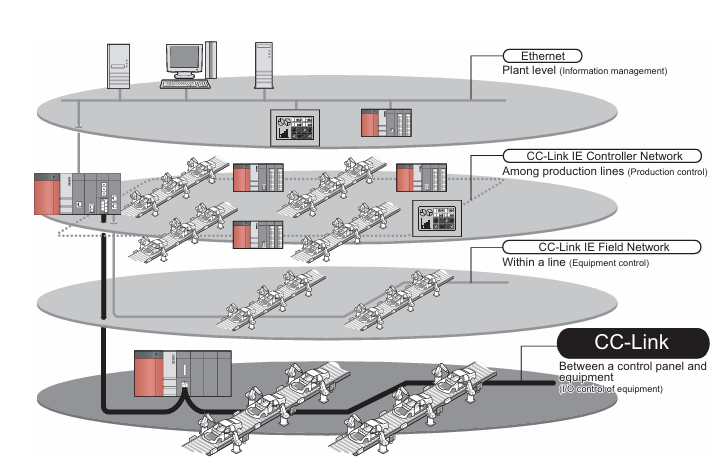
\includegraphics[width=0.7\textwidth]{figures/Chapter2/cc-link2.png}
    \caption{Cấu trúc mạng CC-Link}
    \label{fig:cclink_structure}
\end{figure}

%==============================================================================================================================
\subsection{Master/Local Modules}

Dòng PLC MELSEC-Q có thể giao tiếp với nhau hoặc với các thiết bị ngoại vi thông qua CC-Link nhờ các module Master/Local. Các trạm PLC trong mạng có thể được điều khiển như đang nằm trên cùng một base unit.

Các tính năng chính của hệ thống CC-Link:

\begin{enumerate}
    % ------------------- 1 -------------------
    \item \textbf{Truyền thông dữ liệu chu kỳ và truyền thông tức thời}  
    Master/Local Modules có thể trao đổi dữ liệu theo hai phương thức:
    \begin{itemize}
        \item \textit{Cyclic Transmission}: truyền liên tục theo chu kỳ quét của PLC.
        \item \textit{Transient Transmission}: chỉ truyền khi có yêu cầu.
    \end{itemize}

 \begin{figure}[h]
    \centering
    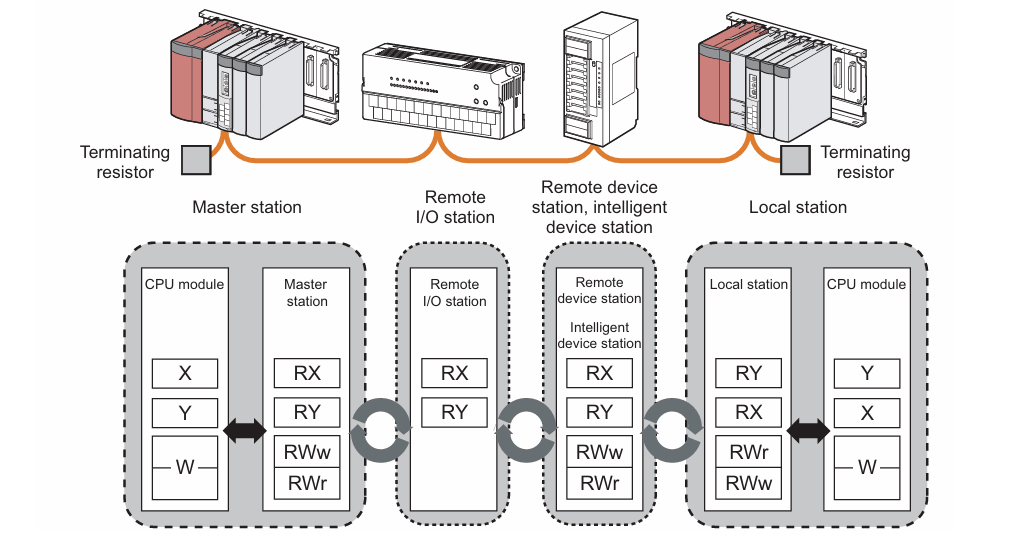
\includegraphics[width=0.48\textwidth]{figures/Chapter01/cclink3.png}
    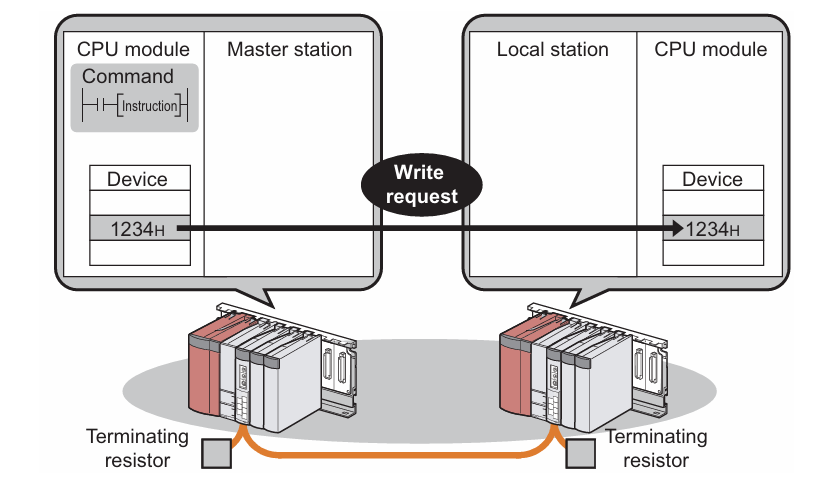
\includegraphics[width=0.48\textwidth]{figures/Chapter01/cclink4.png}
    \caption{Cyclic Transmission và Transient Transmission trong CC-Link}
    \label{fig:cclink_two}
\end{figure}


    % ------------------- 2 -------------------
    \item \textbf{Thiết lập tham số và chẩn đoán hệ thống}  
    Các tham số của module có thể được thiết lập bằng phần mềm GX Works2 hoặc bằng chính chương trình PLC. Khi thiết lập tham số từ chương trình PLC, có thể thay đổi cấu hình mà không cần reset CPU (Hình \ref{fig:cclink_config}).  
    Trạng thái hệ thống, vị trí lỗi và nguyên nhân lỗi có thể được quan sát trực tiếp trên phần mềm lập trình (Hình \ref{fig:cclink_config}).

    \begin{figure}[h]
        \centering
        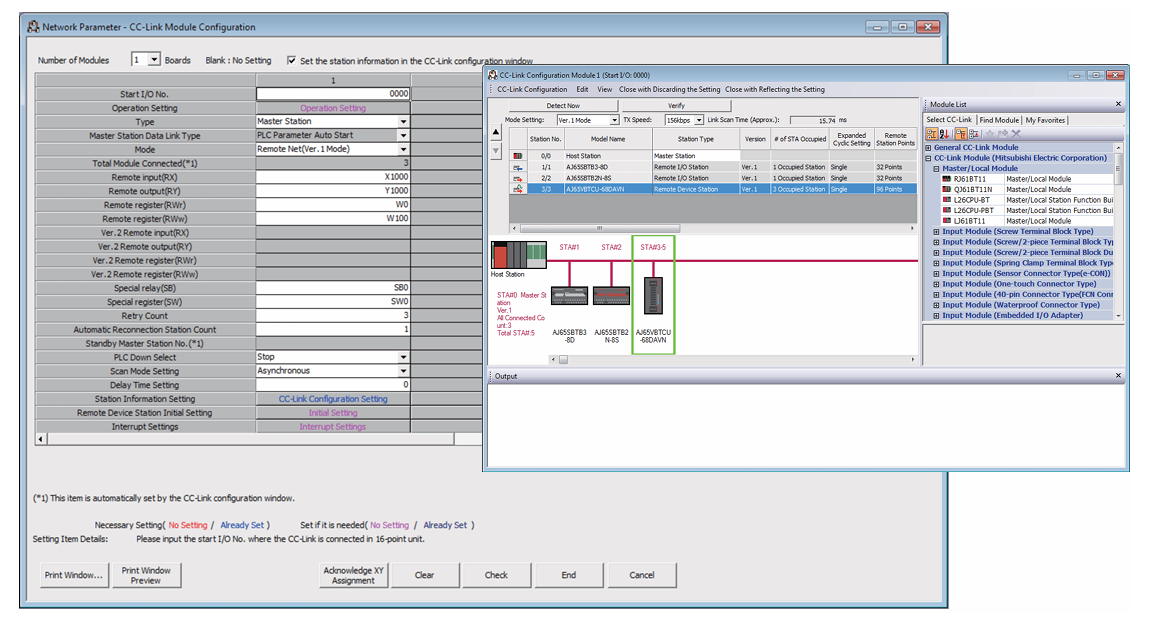
\includegraphics[width=0.48\textwidth]{figures/Chapter01/cclink5.png}
        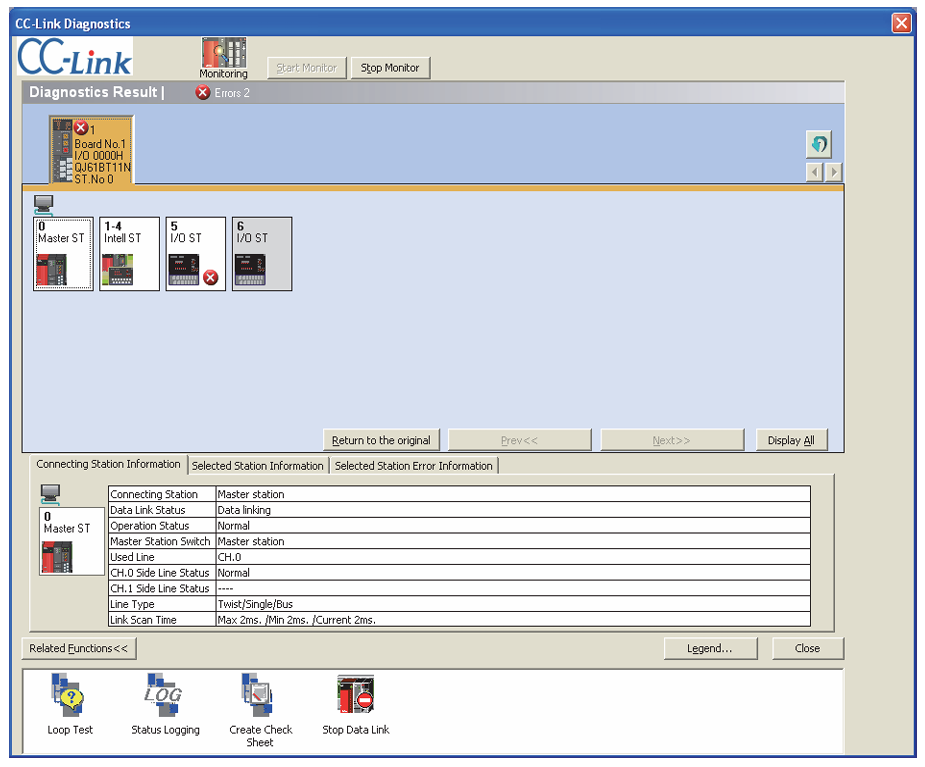
\includegraphics[width=0.48\textwidth]{figures/Chapter01/cclink6.png}
        \caption{Thiết lập tham số module CC-Link}
        \label{fig:cclink_config}
    \end{figure}


    % ------------------- 3 -------------------
    \item \textbf{Hỗ trợ CC-Link Ver.2}  
    Vì Master/Local Module hỗ trợ CC-Link Ver.2, số điểm I/O tối đa trong toàn hệ thống có thể tăng lên:
    \begin{itemize}
        \item 8192 điểm RX/RY,
        \item 2048 word RWr/RWw,
    \end{itemize}
    và theo từng trạm có thể đạt:
    \begin{itemize}
        \item 896 điểm RX/RY,
        \item 128 word RWr/RWw.
    \end{itemize}

    CC-Link Ver.2 có khả năng mở rộng lớn hơn đáng kể so với Ver.1 (Hình \ref{fig:cclink_ver2}).

    \begin{figure}[h]
        \centering
        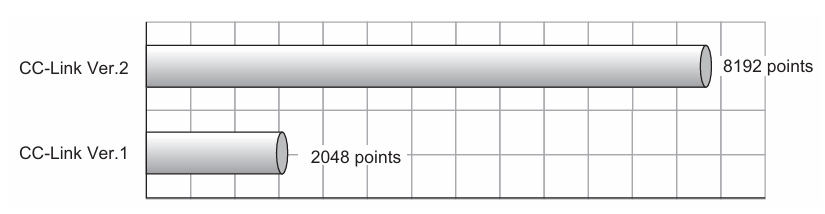
\includegraphics[width=0.7\textwidth]{figures/Chapter01/cclink7.png}
        \caption{So sánh khả năng mở rộng giữa CC-Link Ver.1 và Ver.2}
        \label{fig:cclink_ver2}
    \end{figure}

    % ------------------- 4 -------------------
    \item \textbf{Phòng ngừa sự cố hệ thống}  
    Nhờ cấu trúc nối bus, hệ thống vẫn tiếp tục truyền thông bình thường ngay cả khi một module gặp lỗi. Sau khi module được thay thế hoặc sửa chữa, hệ thống hoạt động trở lại mà không cần cấu hình lại.

\end{enumerate}

%==========================================================================================================
\subsection{Module QJ61BT11N}

Module QJ61BT11N là module Master/Local CC-Link dành cho PLC MELSEC-Q Series \cite{mitsubishi_qj61bt11n_manual}. Hình dạng mặt trước của module được minh họa trong Hình \ref{fig:qj61bt11n}.


\begin{figure}
    \centering
    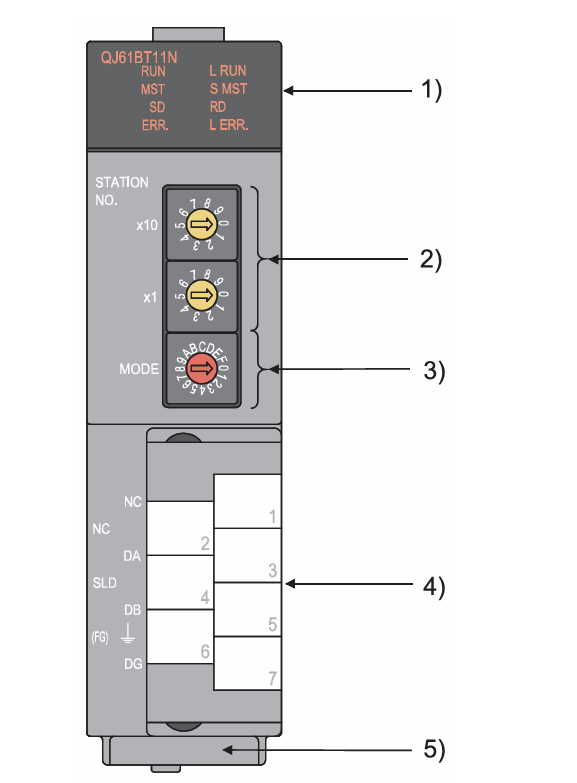
\includegraphics[width=0.5\linewidth]{figures/Chapter01/qj61bt11n.png}
    \caption{Module QJ61BT11N (Master/Local CC-Link)}
    \label{fig:qj61bt11n}
\end{figure}

Các thành phần chính ở mặt trước module gồm:
\begin{itemize}
    \item (1) Đèn LED hiển thị trạng thái,
    \item (2) Thiết lập số thứ tự trạm,
    \item (3) Thiết lập tốc độ truyền thông,
    \item (4) Cổng kết nối cáp CC-Link,
    \item (5) Mã số Serial Number của module.
\end{itemize}

Để cấu hình module CC-Link giao tiếp cần cấu hình địa chỉ của trạm (0 nếu là trạm Master) và Mode (tốc độ truyền nhận). 

% =======================
% PHẦN 3: HỆ CHUYỂN ĐỘNG SERVO
% =======================
\section{Servo motor và Module QD77MS16}

%=======================================================================================
\subsection{Servo và Servo Amplifier}

Servo (bao gồm servo motor và servo amplifier) là hệ truyền động được sử dụng phổ biến trong tự động hóa để điều khiển vị trí, tốc độ và mô-men xoắn với độ chính xác cao. Không giống động cơ thường, servo được trang bị encoder hoặc cảm biến hồi tiếp để thực hiện điều khiển vòng kín (closed-loop control). Nhờ vậy, servo có khả năng đáp ứng nhanh, sai số nhỏ và độ ổn định cao, phù hợp cho các ứng dụng yêu cầu độ chính xác như máy CNC, robot công nghiệp, dây chuyền sản xuất linh kiện điện tử, đóng gói và in ấn.

Một hệ thống servo bao gồm:  
(1) Servo motor,  
(2) Servo amplifier/driver,  
(3) Bộ điều khiển (PLC hoặc motion controller).  
Servo amplifier nhận lệnh từ bộ điều khiển, xử lý phản hồi từ encoder và điều chỉnh dòng điện cấp cho motor để bảo đảm vận hành đúng quỹ đạo đặt trước.

Trong hệ thống này, động cơ sử dụng là \textbf{HG-KR32} kết hợp với \textbf{servo amplifier MR-J4-20B}. Ngoài ra, Mitsubishi Electric cung cấp nhiều dải công suất và chủng loại servo khác nhau phù hợp cho nhiều ứng dụng công nghiệp.

% ---------------- Two images side-by-side ----------------
\begin{figure}[h]
    \centering
    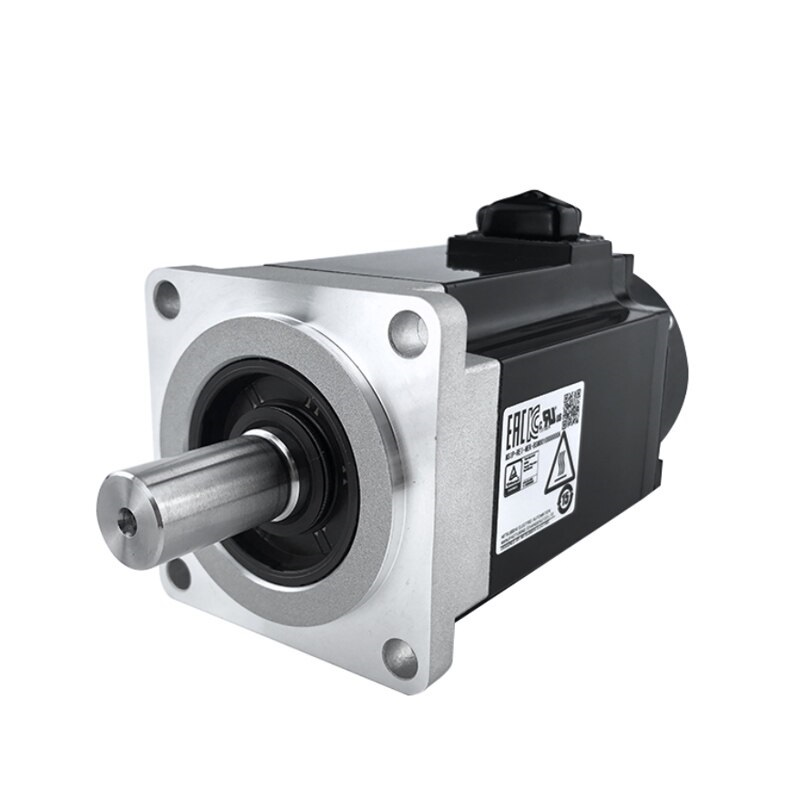
\includegraphics[width=0.48\linewidth]{figures/Chapter01/servo.jpg}
    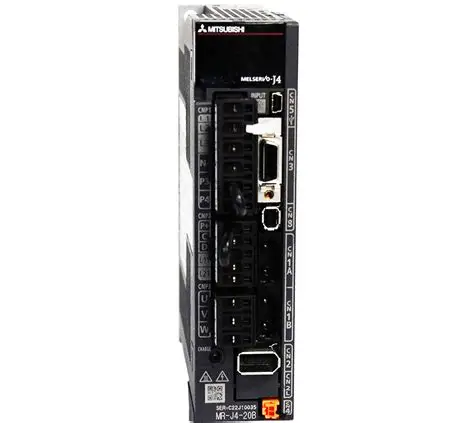
\includegraphics[width=0.48\linewidth]{figures/Chapter01/mrj420b.png}
    \caption{Bộ truyền động servo sử dụng trong hệ thống}
    \label{fig:servo_system}
\end{figure}
% ----------------------------------------------------------

Cấu hình của Driver điều khiển cần đúng với thông số của động cơ Servo.

%===========================================================================================
\subsection{Module QD77MS16}

\textbf{QD77MS16} (Hình \ref{fig:qd77ms}) là module điều khiển chuyển động (Simple Motion Module) thuộc dòng PLC MELSEC-Q của Mitsubishi Electric \cite{mitsubishi_qd77ms_manual}. Module được thiết kế để thực hiện các bài toán điều khiển vị trí, tốc độ và mô-men với độ chính xác cao, hỗ trợ đồng bộ nhiều trục trong hệ thống tự động hóa hiện đại.

\begin{figure}[h]
    \centering
    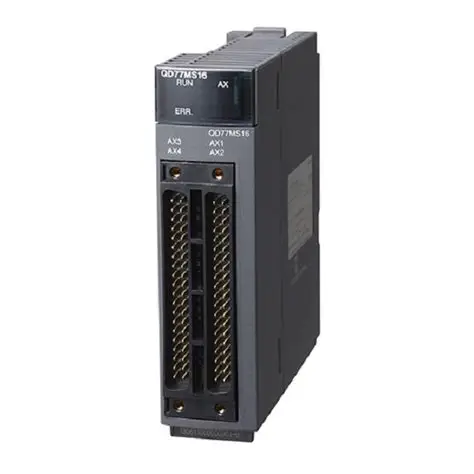
\includegraphics[width=0.42\linewidth]{figures/Chapter01/qd77ms16.png}
    \caption{Module điều khiển chuyển động QD77MS16}
    \label{fig:qd77ms}
\end{figure}

\textbf{Các đặc điểm chính của QD77MS16:}

\begin{itemize}
    \item \textbf{Thời gian khởi động nhanh:}  
    Đạt 0.88 ms (với QD77MS4) trong chế độ điều khiển định vị.

    \item \textbf{Nhiều chức năng điều khiển định vị:}  
    Hỗ trợ điều khiển HPR, điều khiển vị trí, điều khiển tốc độ, chuyển đổi vị trí--tốc độ và điều khiển bằng tay.
    \begin{itemize}
        \item 6 phương pháp HPR khác nhau, hỗ trợ cơ chế HPR retry.  
        \item Điều khiển độc lập từng trục hoặc nội suy 2--4 trục.  
        \item Điều khiển tốc độ--mô-men không qua vòng vị trí.  
        \item Tối đa 600 bộ dữ liệu định vị cho mỗi trục.  
        \item Hỗ trợ thực thi liên tiếp nhiều khối dữ liệu định vị.  
        \item Hai dạng gia tốc/giảm tốc: tuyến tính (trapezoidal) và cong S.  
    \end{itemize}

    \item \textbf{Điều khiển đồng bộ và cam điện tử (E-Cam).}

    \item \textbf{Chức năng phát hiện mark:}  
    Có khả năng latch dữ liệu theo tín hiệu từ DI1--DI4, phù hợp với các ứng dụng cắt theo mark hoặc đồng bộ in ấn.

    \item \textbf{Khả năng bảo trì cao:}  
    Dữ liệu được lưu trong flash ROM, không yêu cầu pin.  
    Thông tin lỗi được lưu và truy xuất trực tiếp từ CPU PLC.

    \item \textbf{Hỗ trợ lệnh chuyên dụng:}  
    Bao gồm Positioning Start, Teaching, và các lệnh tương thích LD77MH/QD75MH giúp tái sử dụng chương trình cũ.

    \item \textbf{Thiết lập và giám sát qua GX Works2:}  
    Dễ dàng cấu hình tham số, kiểm tra wiring, chạy thử, giám sát và debug hệ thống.  
    Có thể kết hợp với \textbf{MR Configurator2} để cấu hình chi tiết servo.

    \item \textbf{Kết nối tốc độ cao qua mạng SSCNET III/H:}  
    Tương thích với MR-J5-B, MR-J4-B, MR-J3-B, MR-JE-B(F), hỗ trợ truyền quang tốc độ cao, giảm nhiễu;  
    cho phép đọc/ghi tham số servo trực tiếp từ module.

    \item \textbf{Hệ thống vị trí tuyệt đối (Absolute Position System):}  
    Sử dụng với MR-J5/J4/J3, chỉ cần gắn pin absolute vào amplifier, không cần proximity dog;  
    khi bật nguồn lại không cần thực hiện HPR.
\end{itemize}


% =======================
% PHẦN 4: ROBOT CÔNG NGHIỆP
% =======================
\section{Robot công nghiệp}

Trong bối cảnh tự động hóa và công nghiệp 4.0 phát triển mạnh, robot công nghiệp, đặc biệt là robot dạng cánh tay, được ứng dụng rộng rãi nhằm tăng năng suất, cải thiện chất lượng và giảm chi phí lao động.

%=====================================================================================
\subsection{Hệ thống Robot Yaskawa}

Một hệ thống robot Yaskawa cơ bản gồm bộ điều khiển (controller), tay máy (manipulator), thiết bị điều khiển cầm tay (programming pendant) và các cáp kết nối.

\begin{itemize}
    \item Cáp programming pendant: kết nối thiết bị cầm tay với bộ điều khiển.
    \item Cáp manipulator: kết nối bộ điều khiển với tay máy, truyền tín hiệu servo và nguồn.
    \item Cáp cấp nguồn: cấp điện (1 pha hoặc 3 pha), yêu cầu có bộ lọc nhiễu.
\end{itemize}

Sơ đồ kết nối tổng quát của hệ thống robot thể hiện trên Hình \ref{fig:yaskawa-dia}.

\begin{figure}[H]
    \centering
    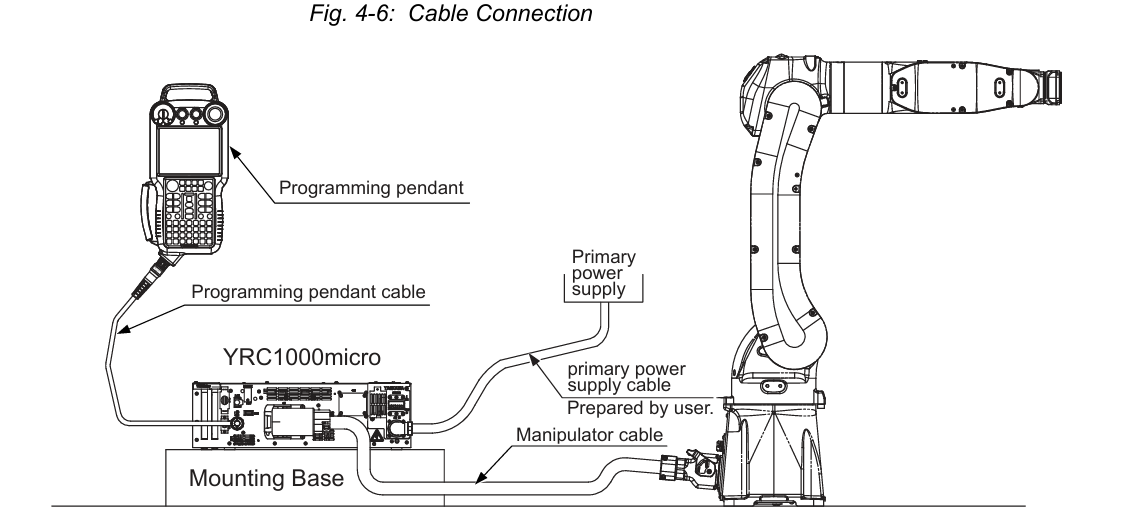
\includegraphics[width=0.75\textwidth]{figures/Chapter2/yaskawa-diagram.png}
    \caption{Sơ đồ tổng quát hệ thống robot công nghiệp}
    \label{fig:yaskawa-dia}
\end{figure}

Hệ thống tại phòng thực hành sử dụng tay máy GP7 và bộ điều khiển YRC1000micro.

% -------------------- GP7 --------------------
\subsubsection{Tay máy GP7}

Robot Yaskawa GP7 (Hình \ref{c2:gp7}) là robot sáu trục với tải trọng 7\,kg, kích thước nhỏ gọn, phù hợp các ứng dụng gắp–đặt, lắp ráp và kiểm tra. GP7 có tốc độ cao, độ chính xác lặp lại khoảng \(\pm 0.01\,\mathrm{mm}\) và dễ lập trình thông qua bộ điều khiển YRC1000micro.

\begin{figure}[H]
    \centering
    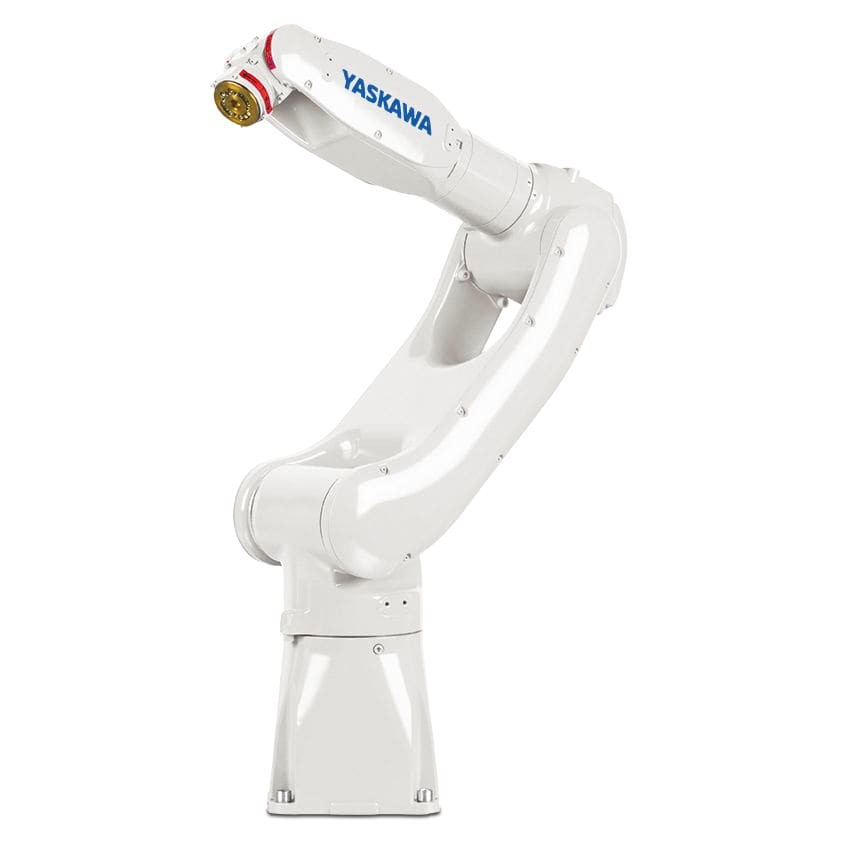
\includegraphics[width=0.5\textwidth]{figures/Chapter2/gp7.jpg}
    \caption{Tay máy GP7}
    \label{c2:gp7}
\end{figure}

Thông số chính:
\begin{itemize}
    \item Tải trọng: 7\,kg
    \item Tầm với ngang: 927\,mm
    \item Tầm với dọc: 1693\,mm
    \item Độ chính xác lặp lại: \(\pm 0.01\,\mathrm{mm}\)
\end{itemize}

Bảng \ref{tab:gp7_axes} trình bày phạm vi chuyển động theo từng trục.

\begin{table}[H]
\centering
\begin{tabularx}{\textwidth}{|c|X|c|c|}
\hline
Trục & Phạm vi (°) & Tốc độ (°/s) & Moment (N·m) \\ \hline
S & \(\pm 170\) & 375 & - \\ \hline
L & \(+145/-65\) & 315 & - \\ \hline
U & \(+190/-70\) & 410 & - \\ \hline
R & \(\pm 190\) & 550 & 17 \\ \hline
B & \(\pm 135\) & 550 & 17 \\ \hline
T & \(\pm 360\) & 1000 & 10 \\ \hline
\end{tabularx}
\caption{Phạm vi chuyển động các trục robot GP7}
\label{tab:gp7_axes}
\end{table}


% -------------------- YRC1000micro --------------------
\subsubsection{Bộ điều khiển YRC1000micro}

\begin{figure}[H]
    \centering
    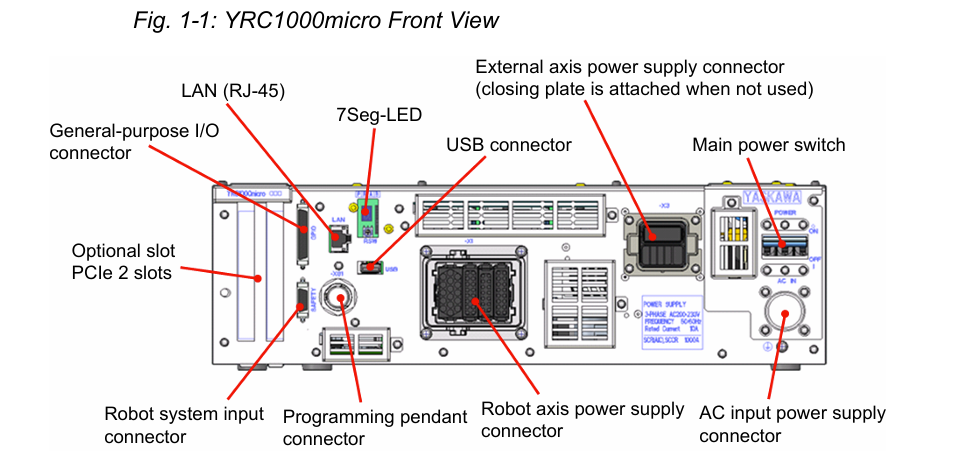
\includegraphics[width=0.75\textwidth]{figures/Chapter2/yrc1000micro.png}
    \caption{Bộ điều khiển YRC1000micro}
    \label{fig:yrc1000}
\end{figure}

Các thành phần chính ở mặt trước controller:

\begin{itemize}
    \item AC input power connector: kết nối nguồn cấp.
    \item Main power switch: bật/tắt nguồn hệ thống.
    \item Robot axis power connector: cấp nguồn và tín hiệu servo cho robot.
    \item USB connector: lưu chương trình/backup dữ liệu.
    \item Programming pendant connector: kết nối pendant.
    \item LAN RJ-45: truyền thông Ethernet/IP.
    \item General-purpose I/O connector: kết nối cảm biến, nút nhấn, relay.
    \item Safety input connector: kết nối tín hiệu an toàn (cửa, dừng khẩn).
\end{itemize}

% -------------------- Pendant --------------------
\subsubsection{Giao diện Teaching Pendant}

Hình \ref{c2:img1} minh họa giao diện chính của pendant.

\begin{figure}[H]
    \centering
    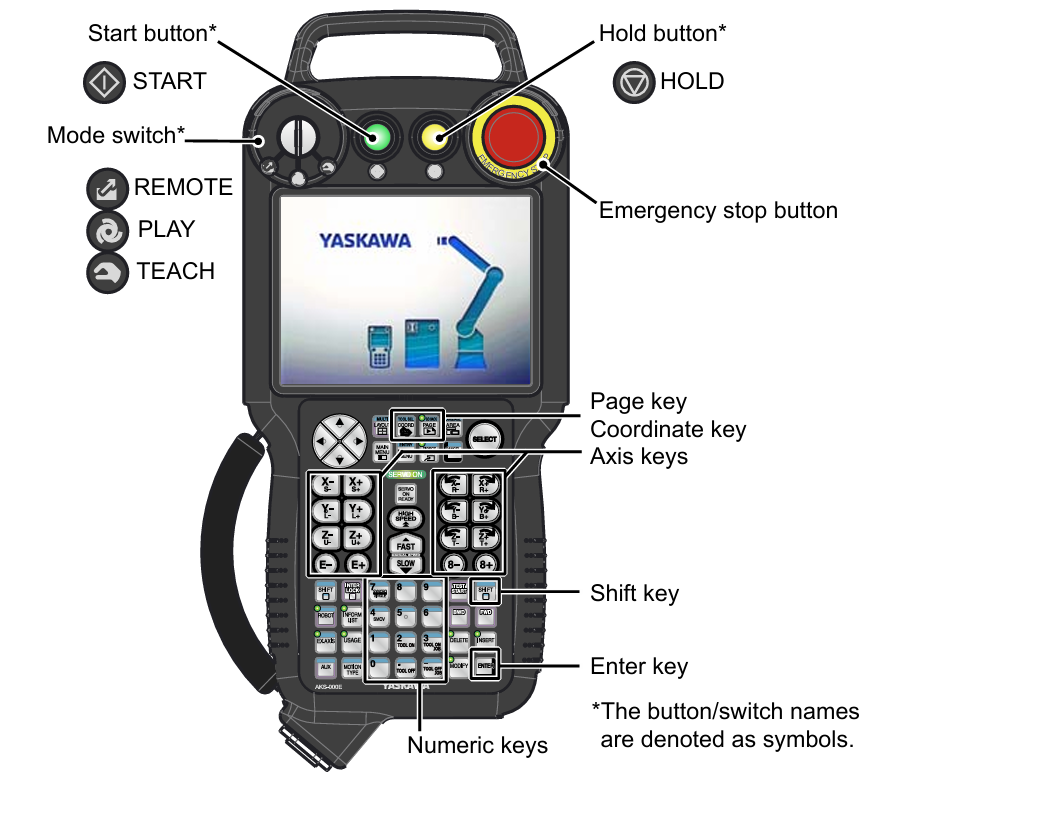
\includegraphics[width=1\textwidth]{figures/Chapter2/image1.png}
    \caption{Giao diện Teach pendant}
    \label{c2:img1}
\end{figure}

\begin{longtable}{|p{0.30\textwidth}|p{0.70\textwidth}|}
\hline
Mục & Mô tả \\ \hline
Phím ký tự / biểu tượng & Các phím như [ENTER]. \\ \hline
Phím trục / phím số & Dùng điều khiển trục hoặc nhập giá trị. \\ \hline
Nhấn đồng thời & Ví dụ [SHIFT]+[COORD]. \\ \hline
Công tắc chế độ & Chọn REMOTE, PLAY hoặc TEACH. \\ \hline
Nút bấm & START, HOLD, EMERGENCY STOP. \\ \hline
Màn hình hiển thị & Các mục menu viết dạng \{JOB\}. \\ \hline
\end{longtable}

% -------------------- Viết chương trình --------------------
Điều kiện trước khi dạy robot: nút \texttt{Emergency Stop} không được nhấn, pendant ở chế độ \texttt{TEACH}, bật nguồn \texttt{SERVO} và giữ công tắc trên tay cầm.

Để tạo chương trình mới:  
\texttt{MAIN MENU} → \texttt{JOB} → \texttt{CREATE NEW JOB} → đặt tên → \texttt{EXECUTE}.

\begin{figure}[H]
    \centering
    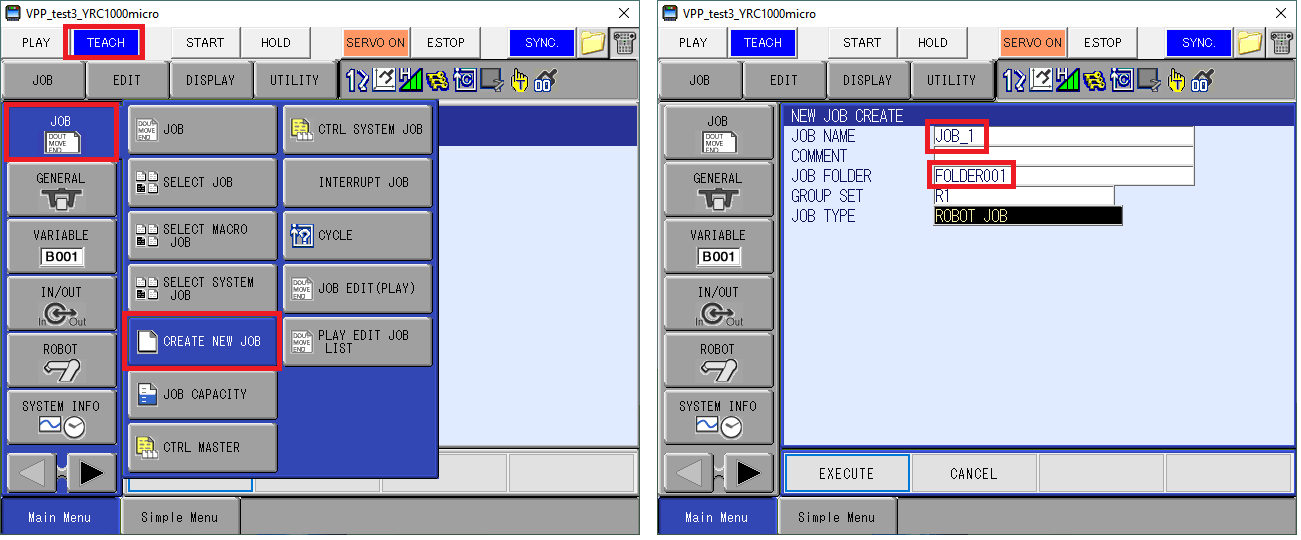
\includegraphics[width=1\textwidth]{figures/Chapter2/yaskawa-process.png}
    \caption{Tạo chương trình mới bằng pendant}
    \label{c2:yakawa-process}
\end{figure}

Màn hình viết chương trình được hiển thị như Hình \ref{c2:job}.

\begin{figure}[H]
    \centering
    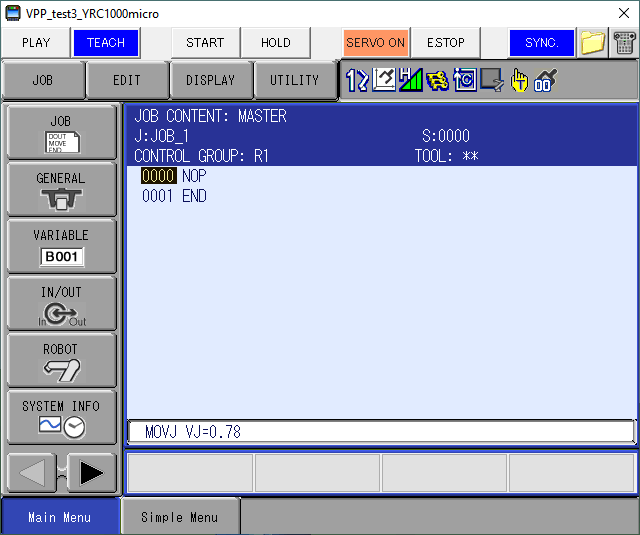
\includegraphics[width=0.75\textwidth]{figures/Chapter2/job.png}
    \caption{Màn hình tạo Job}
    \label{c2:job}
\end{figure}

Cấu trúc một lệnh trong INFORM III gồm:
\begin{center}
\texttt{MOVJ \quad VJ=50.00}
\end{center}

\begin{itemize}
    \item \textbf{Instruction}: loại lệnh cần thực hiện.
    \item \textbf{Additional item}: điều kiện hoặc tham số kèm theo.
\end{itemize}

Các nhóm lệnh trong INFORM III được trình bày trong Bảng \ref{tab:inform-types}.

\begin{table}[H]
\centering
\begin{tabular}{|p{0.30\textwidth}|p{0.68\textwidth}|}
\hline
Loại lệnh & Nội dung \\ \hline
I/O Instruction & Điều khiển tín hiệu I/O \\ \hline
Control Instruction & Điều khiển luồng chương trình \\ \hline
Operating Instruction & Thao tác với biến \\ \hline
Move Instruction & Điều khiển chuyển động của robot \\ \hline
Shift Instruction & Dịch chuyển điểm dạy \\ \hline
Adheres Instruction & Lệnh đi kèm \\ \hline
Work Instruction & Lệnh liên quan thao tác công việc \\ \hline
Optional Instruction & Chức năng tùy chọn \\ \hline
\end{tabular}
\caption{Các nhóm lệnh trong INFORM III}
\label{tab:inform-types}
\end{table}


%===========================================================================================
\subsection{Hệ thống robot Hyundai}

Hệ thống robot Hyundai gồm tay máy và bộ điều khiển, mô tả trong Hình \ref{fig:hyun1}.

\begin{figure}[H]
    \centering
    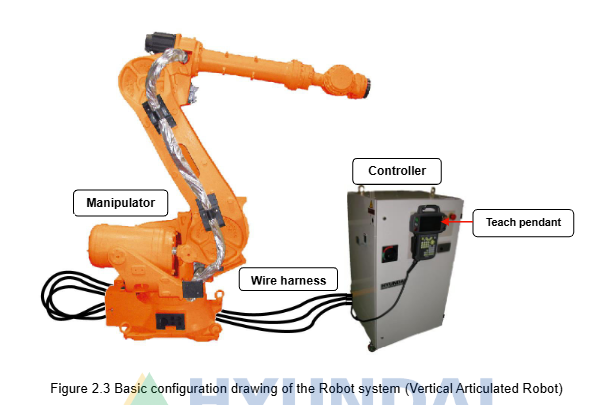
\includegraphics[width=1\textwidth]{figures/Chapter2/hyundai-diagram}
    \caption{Hệ thống robot Hyundai cơ bản}
    \label{fig:hyun1}
\end{figure}

Robot sử dụng là HH7, điều khiển bằng bộ Hi5a.

\begin{figure}[H]
    \centering
    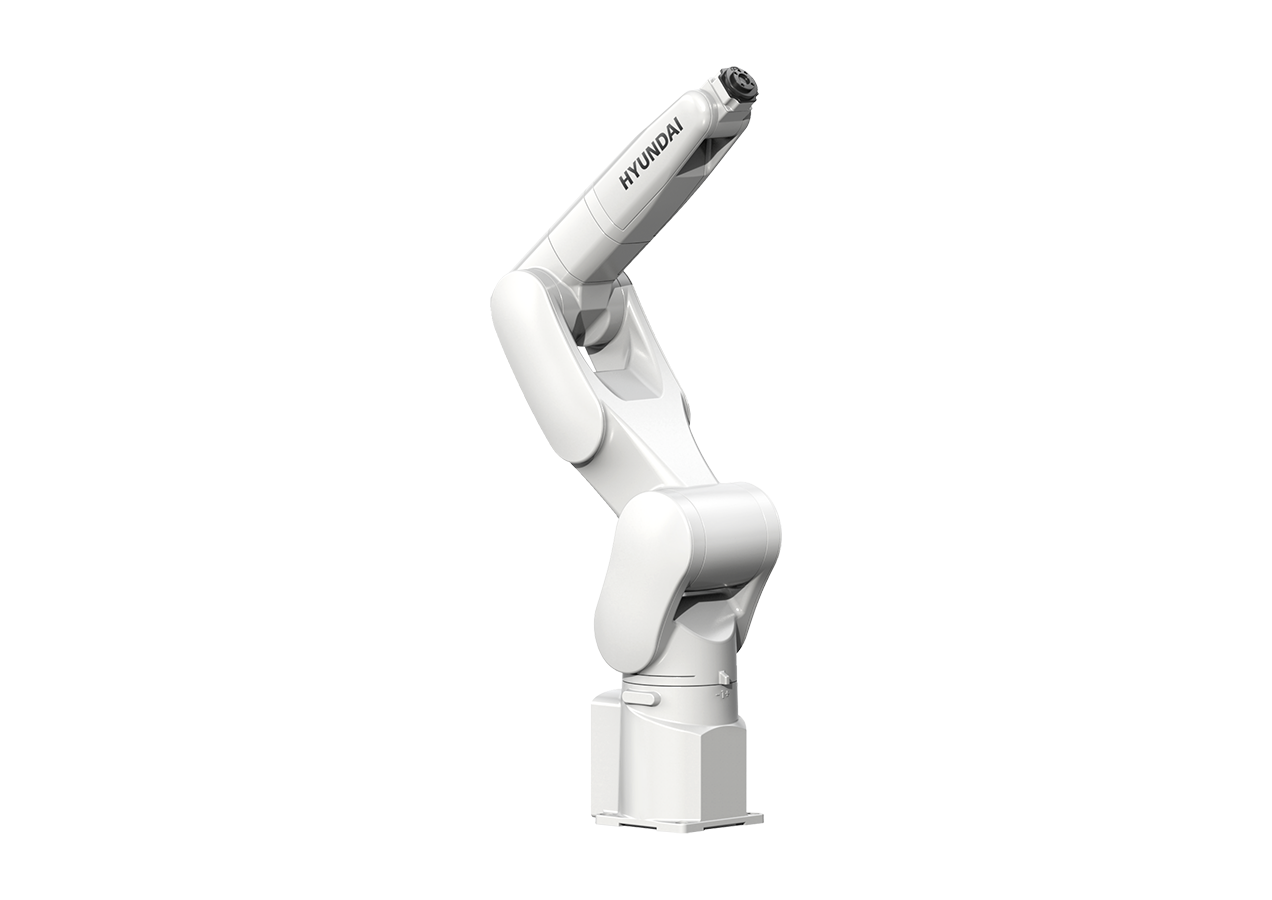
\includegraphics[width=0.6\textwidth]{figures/Chapter2/HH7.png}
    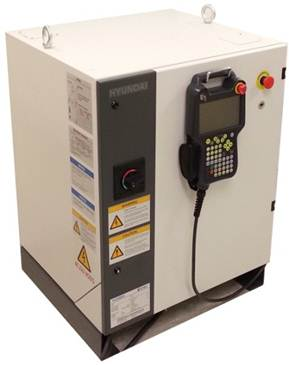
\includegraphics[width=0.3\textwidth]{figures/Chapter2/hi5a.jpg}
    \caption{Tay máy HH7 và Bộ điều khiển Hi5a}
    \label{fig:hyun2}
\end{figure}

Teach pendant của Hi5a có chức năng tương tự pendant của Yaskawa.

\subsubsection{Viết chương trình điều khiển bằng pendant}

Chọn chương trình bằng [SHIFT] + [PROG]. Danh sách chương trình hiển thị như Hình \ref{fig:hyun4}.

\begin{figure}[H]
    \centering
    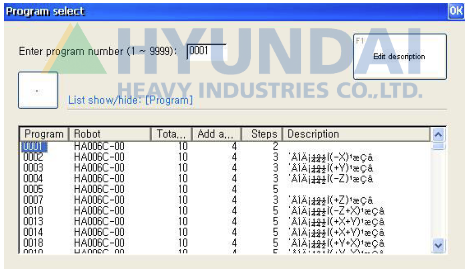
\includegraphics[width=0.75\textwidth]{figures/Chapter2/hyun4.png}
    \caption{Chọn chương trình trên pendant Hi5a}
    \label{fig:hyun4}
\end{figure}

Lệnh robot gồm hai loại:
\begin{itemize}
    \item Lệnh bước: điều khiển chuyển động.
    \item Lệnh chức năng: thực hiện thao tác.
\end{itemize}

\begin{figure}[H]
    \centering
    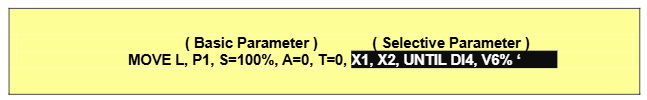
\includegraphics[width=0.75\textwidth]{figures/Chapter2/command.png}
    \caption{Ví dụ một lệnh cơ bản}
    \label{fig:hyun5}
\end{figure}

Mỗi lệnh gồm phần command và các thuộc tính (properties), chia thành:
\begin{itemize}
    \item Thuộc tính bắt buộc.
    \item Thuộc tính tùy chọn.
\end{itemize}

Khi chỉnh sửa, người dùng có thể nhập số, chọn từ menu hoặc nhập ký tự.



% =======================
% PHẦN 4: COMPUTER VISION
% =======================
\section{Thị giác máy tính và mô hình YOLO}
%=======================================================================
\subsection{Thị giác máy tính}
Thị giác máy tính (Computer Vision) là lĩnh vực nghiên cứu cách máy tính hiểu và diễn giải hình ảnh hoặc video, tương tự như cách con người nhận thức thị giác. Trong công nghiệp, thị giác máy đóng vai trò quan trọng trong tự động hóa các tác vụ kiểm tra, giám sát và điều khiển chất lượng.

Một trong những ứng dụng phổ biến nhất của thị giác máy tính là kiểm tra sản phẩm trên dây chuyền sản xuất. Hệ thống camera thu thập hình ảnh sản phẩm, sau đó sử dụng thuật toán xử lý ảnh để phát hiện lỗi như thiếu linh kiện, lắp sai hướng, sai vị trí hoặc khuyết tật bề mặt. So với kiểm tra thủ công, thị giác máy có ưu thế vượt trội về tốc độ, độ chính xác và khả năng hoạt động liên tục.

Ngoài kiểm tra chất lượng, thị giác máy còn được ứng dụng trong các nhiệm vụ như:
\begin{itemize}
    \item \textbf{Nhận dạng ký tự quang học (OCR):} đọc mã bưu chính viết tay trên thư và nhận dạng biển số xe tự động.
    \item \textbf{Kiểm tra máy (Machine inspection):} kiểm tra nhanh các chi tiết để đảm bảo chất lượng bằng stereo vision với hệ thống chiếu sáng chuyên dụng để đo sai số dung sai trên cánh máy bay hoặc thân xe ôtô, hoặc phát hiện lỗi trong khuôn đúc thép bằng ảnh X-ray.
    \item \textbf{Bán lẻ:} nhận dạng vật thể cho các quầy thanh toán tự động và cửa hàng hoàn toàn tự động.
    \item \textbf{Logistics kho:} giao hàng tự động, robot chở pallet và robot gắp hàng bằng tay máy trong kho.
    \item \textbf{Ảnh y tế:} ghép ảnh trước và trong phẫu thuật hoặc nghiên cứu dài hạn về sự thay đổi hình thái não khi con người già đi.
    \item \textbf{Xe tự lái:} di chuyển tự động giữa các thành phố và cả bay tự động.
    \item \textbf{Dựng mô hình 3D (photogrammetry):} xây dựng mô hình 3D hoàn toàn tự động từ ảnh chụp trên không và ảnh drone.
    \item \textbf{Match move:} kết hợp hình ảnh CGI với cảnh quay thực bằng cách theo dõi điểm đặc trưng trong video nguồn để ước tính chuyển động camera 3D và hình dạng môi trường. Kỹ thuật này được sử dụng rộng rãi ở Hollywood, ví dụ như trong phim \textit{Jurassic Park}; ngoài ra còn yêu cầu kỹ thuật tách nền chính xác để chèn đối tượng giữa tiền cảnh và hậu cảnh.
    \item \textbf{Ghi chuyển động (Motion capture – mocap):} sử dụng các marker phản quang từ nhiều camera hoặc kỹ thuật thị giác máy tính khác để thu chuyển động diễn viên cho hoạt hình.
    \item \textbf{Giám sát:} phát hiện người xâm nhập, phân tích giao thông đường cao tốc và giám sát hồ bơi để phát hiện người đuối nước.
\end{itemize}


Trong sản xuất điện tử, thị giác máy đặc biệt quan trọng ở khâu kiểm tra AOI/AVI. Các mô hình học sâu hiện đại như CNN, YOLO giúp hệ thống phân loại và phát hiện linh kiện nhanh, chính xác hơn, giảm đáng kể tỷ lệ lỗi do con người.
%===========================================================================
\subsection{Thư viện OpenCV}

OpenCV (Open Source Computer Vision Library) là thư viện mã nguồn mở được sử dụng rộng rãi trong các hệ thống thị giác máy tính và xử lý ảnh thời gian thực. Thư viện hỗ trợ hàng trăm thuật toán cốt lõi, bao gồm xử lý ảnh cơ bản, phát hiện biên, nhận dạng đối tượng, theo dõi chuyển động, hiệu chỉnh camera và nhiều chức năng nâng cao phục vụ cho tự động hóa công nghiệp. Với ưu điểm tốc độ cao, dễ tích hợp và hoạt động tốt trên nhiều nền tảng (C++, Python, CUDA), OpenCV là lựa chọn phổ biến cho các hệ thống AOI, robot, và các ứng dụng thị giác máy tính hiện đại.

\subsubsection*{Các nhóm chức năng chính của OpenCV}

\begin{itemize}
    \item \textbf{Tiền xử lý ảnh (Image Preprocessing):}  
    Bao gồm chuyển đổi không gian màu (RGB, HSV, LAB), lọc nhiễu (\texttt{GaussianBlur}, \texttt{medianBlur}), cân bằng histogram, trích xuất kênh màu và chuẩn hoá dữ liệu ảnh. Các bước này giúp ổn định chất lượng ảnh đầu vào trước khi gửi vào các thuật toán phát hiện.

    \item \textbf{Biến đổi hình học (Geometric Transformations):}  
    Các phép quay, tịnh tiến, co giãn, cắt (crop), warp affine và warp perspective. Đặc biệt quan trọng trong bài toán căn chỉnh ảnh (image alignment) giữa ảnh chụp thực tế và ảnh mẫu (golden template).

    \item \textbf{Phát hiện biên và đặc trưng (Feature Detection \& Description):}  
    OpenCV hỗ trợ nhiều thuật toán như SIFT, ORB, FAST, BRIEF dùng để trích xuất đặc trưng và mô tả ảnh. Các đặc trưng này được sử dụng trong việc căn chỉnh ảnh, ghép ảnh hoặc theo dõi vật thể.

    \item \textbf{Phân đoạn và trích xuất đối tượng (Segmentation):}  
    Bao gồm thresholding, adaptive thresholding, Otsu, watershed và tìm contour. Đây là bước quan trọng trong việc tách bo mạch PCB khỏi nền hoặc xác định biên dạng linh kiện.

    \item \textbf{Biến đổi tần số và phân tích nâng cao:}  
    Hỗ trợ FFT, DCT, bộ lọc Laplacian, Sobel, Canny. Các thuật toán này phục vụ phát hiện cạnh, phân tích cấu trúc ảnh và tăng độ sắc nét.

    \item \textbf{Đọc/ghi và hiển thị ảnh:}  
    Các hàm như \texttt{imread}, \texttt{imwrite}, \texttt{cvtColor}, \texttt{resize} giúp thao tác ảnh nhanh gọn và thống nhất trong toàn bộ pipeline xử lý.
\end{itemize}

\subsubsection*{Vai trò của OpenCV trong hệ thống}

Trong đề tài này, OpenCV đóng vai trò là nền tảng chính cho toàn bộ pipeline xử lý ảnh từ camera. Các nhiệm vụ chính bao gồm:

\begin{itemize}
    \item Tiền xử lý ảnh để ổn định ánh sáng và màu sắc trước khi phân tích.
    \item Căn chỉnh ảnh (alignment) giữa ảnh thực tế và ảnh mẫu bằng SIFT/ORB.
    \item Tách vùng bo mạch (PCB cropping) dựa trên ngưỡng màu hoặc phân tích kênh màu.
    \item Tính toán độ lệch linh kiện (shift checking) sau khi YOLO phát hiện vị trí.
    \item Giao tiếp với UI và pipeline Python thông qua định dạng ảnh tiêu chuẩn.
\end{itemize}

Nhờ OpenCV, hệ thống đạt được tốc độ xử lý cao, khả năng hoạt động thời gian thực và dễ dàng tích hợp với mô hình học sâu (YOLO) trong quá trình phát hiện lỗi linh kiện.

\subsection{Mạng YOLO - Lược sử phát triển}
\begin{figure}
    \centering
    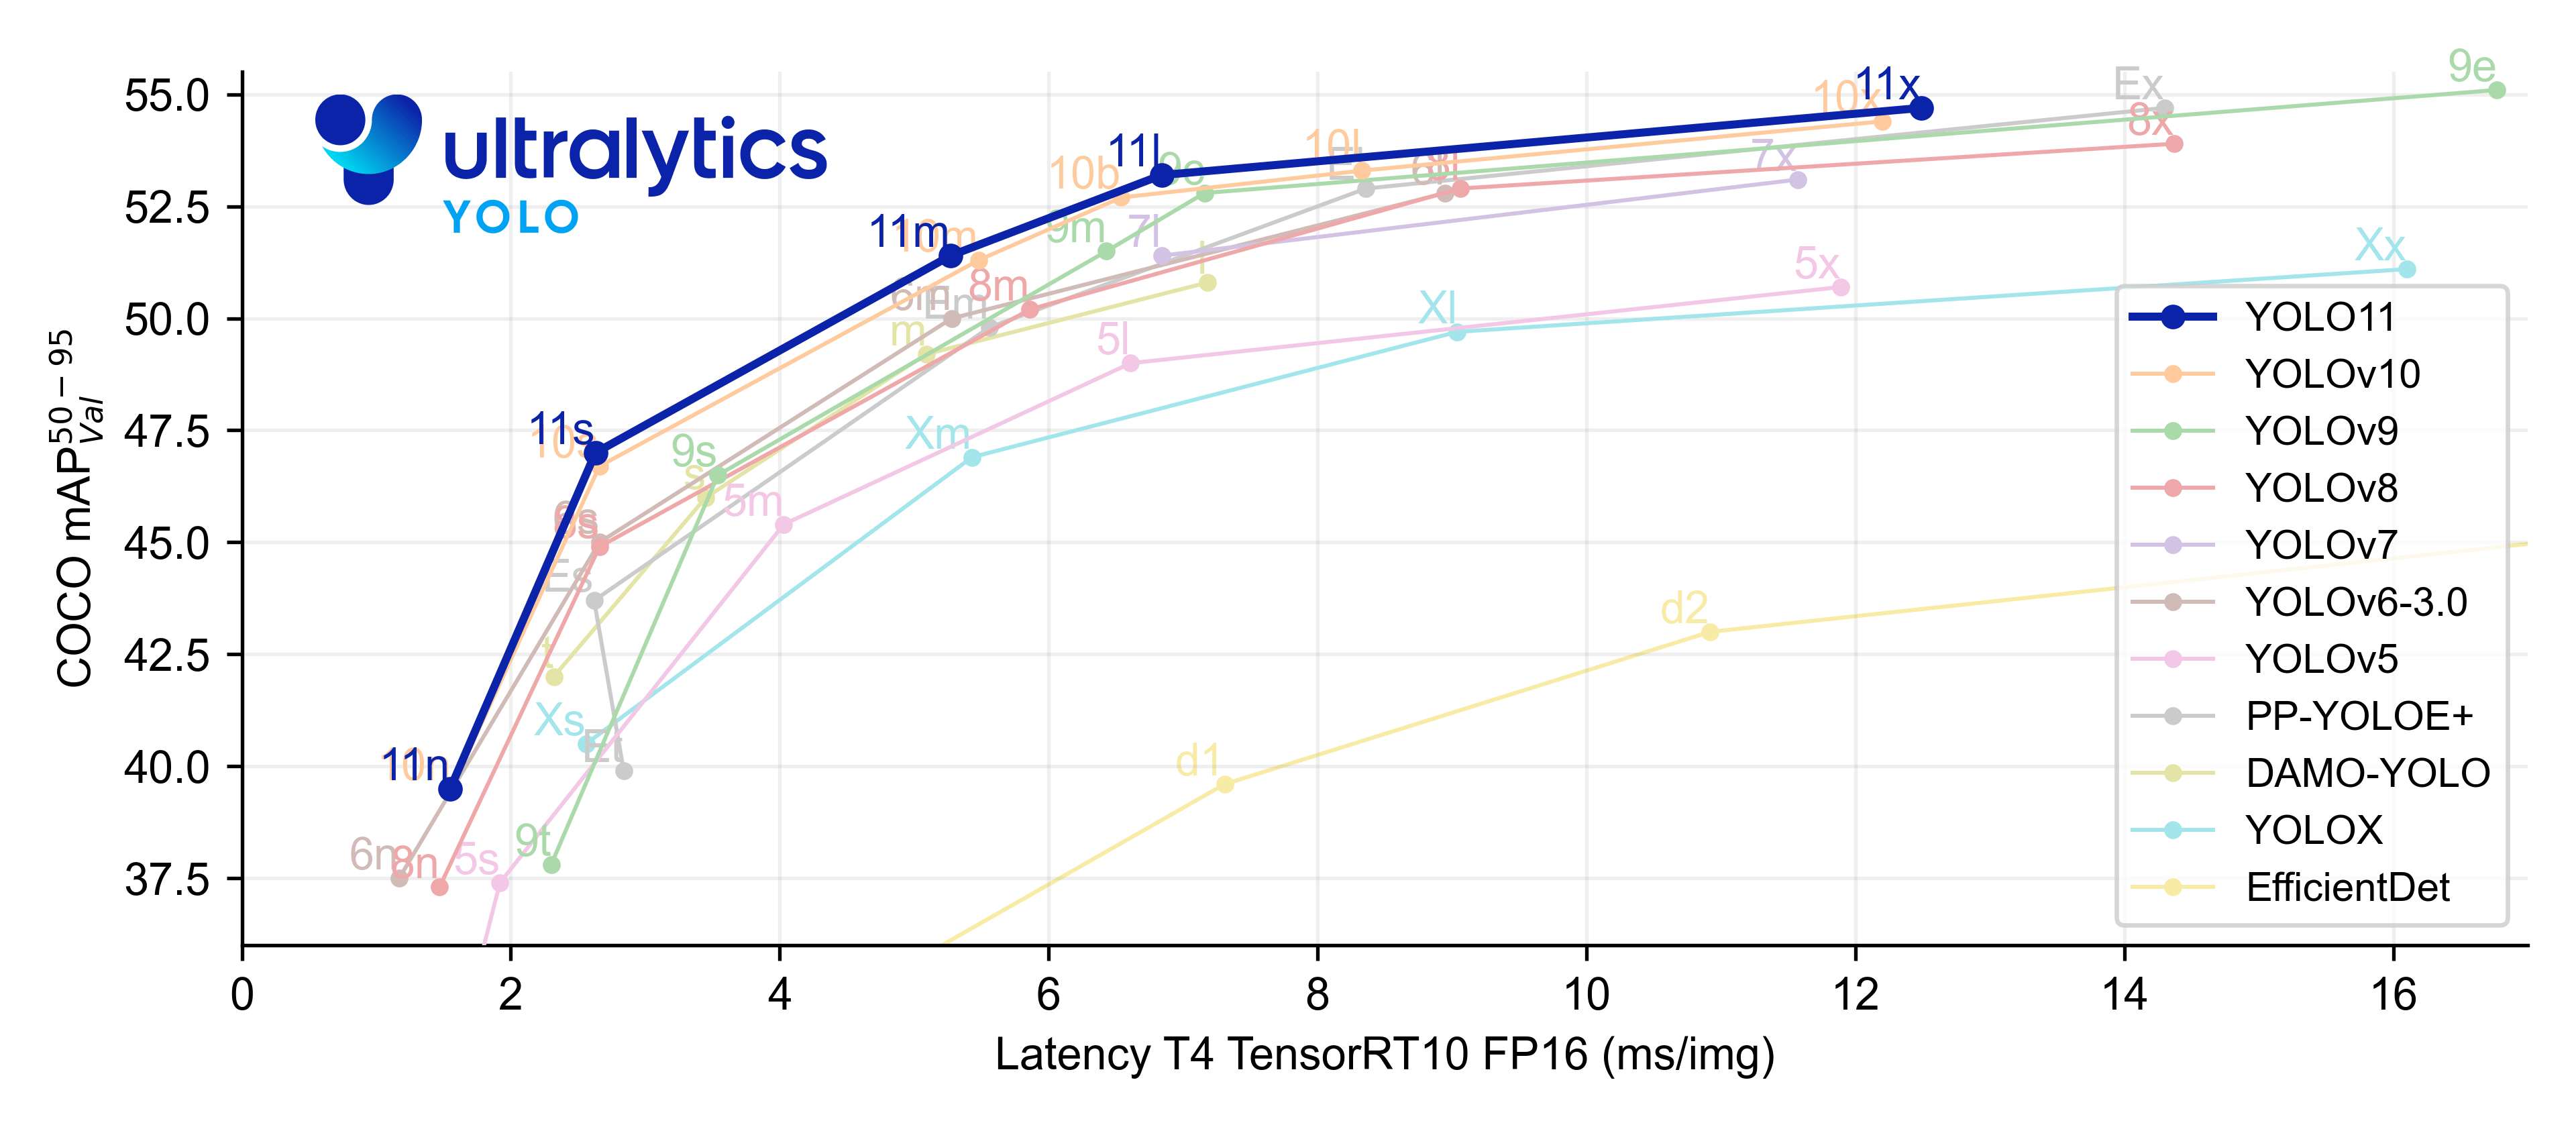
\includegraphics[width=1\textwidth]{figures/Chapter01/performance-comparison.png}
    \caption{YOLO Performance.}
    \label{fig:yolo}
\end{figure}
YOLO (You Only Look Once) là một mô hình nổi tiếng trong lĩnh vực phát hiện đối tượng và phân đoạn ảnh, 
được phát triển bởi Joseph Redmon và Ali Farhadi tại Đại học Washington. 
Ra mắt vào năm 2015, YOLO nhanh chóng được ưa chuộng nhờ tốc độ cao và độ chính xác vượt trội.  

\begin{itemize}
  \item \textbf{YOLOv2 (2016):} Cải tiến so với bản gốc bằng cách bổ sung \textit{batch normalization}, 
  \textit{anchor boxes} và \textit{dimension clusters}.
  
  \item \textbf{YOLOv3 (2018):} Nâng cao hiệu năng với \textit{backbone} hiệu quả hơn, nhiều \textit{anchors} 
  hơn và \textit{spatial pyramid pooling}.
  
  \item \textbf{YOLOv4 (2020):} Giới thiệu các cải tiến như \textit{Mosaic data augmentation}, 
  \textit{anchor-free detection head} và \textit{loss function} mới.
  
  \item \textbf{YOLOv5:} Tiếp tục cải thiện hiệu năng và bổ sung tính năng mới như tối ưu siêu tham số 
  (\textit{hyperparameter optimization}), theo dõi thí nghiệm tích hợp, và tự động xuất ra các định dạng phổ biến.
  
  \item \textbf{YOLOv6 (2022):} Được Meituan phát hành mã nguồn mở, ứng dụng nhiều trong các robot giao hàng tự động.
  
  \item \textbf{YOLOv7:} Mở rộng thêm các tác vụ như ước lượng tư thế (\textit{pose estimation}) trên tập dữ liệu 
  \textit{COCO keypoints}.
  
  \item \textbf{YOLOv8 (2023, Ultralytics):} Bổ sung nhiều tính năng và cải tiến mới, tăng hiệu suất, tính linh hoạt 
  và hiệu quả, đồng thời hỗ trợ đầy đủ các tác vụ thị giác máy tính (\textit{vision AI}).
  
  \item \textbf{YOLOv9:} Giới thiệu phương pháp mới như \textit{Programmable Gradient Information (PGI)} 
  và \textit{Generalized Efficient Layer Aggregation Network (GELAN)}.
  
  \item \textbf{YOLOv10:} Do các nhà nghiên cứu Đại học Thanh Hoa phát triển bằng gói Python của Ultralytics, 
  mang lại tiến bộ trong phát hiện đối tượng thời gian thực nhờ \textit{End-to-End head} loại bỏ nhu cầu sử dụng 
  \textit{Non-Maximum Suppression (NMS)}.
  
  \item \textbf{YOLOv11 (Mới nhất):} Dòng mô hình mới nhất của Ultralytics, đạt hiệu suất tiên tiến 
  (\textit{state-of-the-art}) trên nhiều tác vụ như phát hiện đối tượng, phân đoạn, ước lượng tư thế, 
  theo dõi và phân loại, với khả năng ứng dụng rộng rãi trong nhiều lĩnh vực AI.


\end{itemize}
%====================================================================
\subsection{Ultralytics YOLOv11}
\begin{figure}[h]
    \centering
    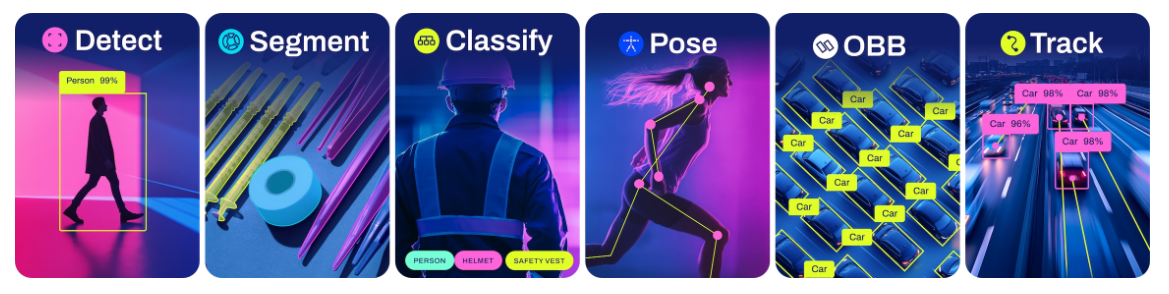
\includegraphics[width=1\textwidth]{figures/Chapter01/yolotasks.png}
    \caption{YOLOv11 Tasks}
    \label{fig:yolov11}
\end{figure}
Ultralytics YOLO11 là một khung AI linh hoạt, hỗ trợ nhiều tác vụ thị giác máy tính khác nhau. Khung này có thể được sử dụng để thực hiện phát hiện đối tượng (detection), phân đoạn ảnh (segmentation), OBB (Oriented Bounding Box), phân loại (classification), và ước lượng tư thế (pose estimation). Mỗi tác vụ có mục tiêu và ứng dụng riêng, cho phép giải quyết nhiều thách thức trong thị giác máy tính chỉ với một framework duy nhất (Hình \ref{fig:yolov11}).

\begin{enumerate}
    \item \textbf{Detection (Phát hiện đối tượng)}: Phát hiện là tác vụ chính được hỗ trợ bởi YOLO11. Nó bao gồm việc xác định các đối tượng trong ảnh hoặc video và vẽ hộp bao quanh (bounding box) chúng. Các đối tượng được phân loại dựa trên đặc trưng. YOLO11 có thể phát hiện nhiều đối tượng trong một ảnh với độ chính xác và tốc độ cao, phù hợp cho các ứng dụng thời gian thực như giám sát an ninh và xe tự hành.
    \item \textbf{Segmentation (Phân đoạn ảnh)}: Phân đoạn chia ảnh thành nhiều vùng dựa trên nội dung, với độ chính xác đến từng pixel. Ứng dụng điển hình gồm chẩn đoán y tế, phân tích nông nghiệp, và kiểm soát chất lượng. YOLO11 triển khai một biến thể của kiến trúc U-Net để đạt hiệu quả cao.
    \item \textbf{Classification (Phân loại ảnh)}: Phân loại gán nhãn cho toàn bộ ảnh dựa trên nội dung. YOLO11 sử dụng biến thể của EfficientNet để đạt hiệu năng cao. Tác vụ này quan trọng trong thương mại điện tử, kiểm duyệt nội dung, và theo dõi động vật hoang dã.
    \item \textbf{Pose Estimation (Ước lượng tư thế)}: Ước lượng tư thế phát hiện các điểm mốc (keypoints) trong ảnh hoặc video để theo dõi chuyển động hoặc ước lượng dáng điệu. Các điểm mốc có thể là khớp cơ thể, đặc điểm khuôn mặt, hoặc các điểm quan trọng khác. YOLO11 cho độ chính xác cao, ứng dụng trong thể dục, phân tích thể thao, và tương tác người–máy.
    \item \textbf{OBB (Oriented Bounding Box – Hộp bao định hướng)}: OBB mở rộng phát hiện đối tượng bằng cách thêm thông tin góc xoay, giúp định vị chính xác các vật thể bị nghiêng hoặc xoay. Điều này đặc biệt hữu ích trong phân tích ảnh hàng không, xử lý tài liệu, và các ứng dụng công nghiệp. YOLO11 hỗ trợ OBB với tốc độ và độ chính xác cao.
\end{enumerate}

%%%%%%%%%%%%%%%%%%%%%%%%%%%%%%%%%%%%%%%%%%%%%%%%%%%%%%%%%%%%%%%
\section{Tổng quan về giao thức OPC UA}

OPC UA (OPC Unified Architecture, IEC 62541) là tiêu chuẩn truyền thông mở được sử dụng rộng rãi trong lĩnh vực tự động hoá công nghiệp. Giao thức cung cấp khả năng trao đổi dữ liệu an toàn, độc lập nền tảng và đáng tin cậy giữa các thiết bị, PLC, robot và các hệ thống phần mềm. OPC UA hỗ trợ cả hai mô hình giao tiếp: client–server và publish/subscribe (PubSub), cho phép triển khai linh hoạt trong nhiều kiến trúc mạng công nghiệp và mạng doanh nghiệp.

OPC UA được phát triển nhằm khắc phục các hạn chế của OPC DA vốn phụ thuộc vào Windows DCOM, không tương thích tốt với tường lửa và thiếu tính mở. Phiên bản đầu tiên của OPC UA được công bố vào năm 2006; phiên bản 1.04 (2017) bổ sung cơ chế PubSub và các chính sách bảo mật nâng cao. Trong đặc tả OPC UA, xác thực, ký số và mã hoá dữ liệu được nhấn mạnh mạnh mẽ trong cả hai mô hình truyền thông.

Với mô hình thông tin tích hợp theo IEC 62541, OPC UA cho phép mô tả dữ liệu, thuộc tính và chức năng của thiết bị theo cấu trúc phân cấp thống nhất. Nhờ đó, OPC UA không chỉ truyền dữ liệu quá trình (set-point, measured value, tham số vận hành) mà còn định nghĩa ý nghĩa của dữ liệu, giúp thiết lập các quy trình giao tiếp hiệu quả giữa PLC và các tầng phần mềm cấp cao như MES hoặc ERP. Các thiết bị trong hệ thống công nghiệp có thể vừa đóng vai trò OPC UA Server vừa là OPC UA Client, hỗ trợ trao đổi dữ liệu ngang và dọc trong dây chuyền.

Trong bối cảnh Industry 4.0 và IIoT, OPC UA được xem là chuẩn truyền thông cốt lõi. Mô hình kiến trúc tham chiếu RAMI 4.0 (2015) khuyến nghị sử dụng OPC UA cho lớp truyền thông, khiến OPC UA trở thành yêu cầu bắt buộc đối với các thiết bị “Industry 4.0-ready”. Ngoài TCP và HTTPS trong mô hình client–server, OPC UA PubSub còn có thể sử dụng UDP, AMQP hoặc MQTT, phù hợp cho các ứng dụng tốc độ cao và mạng phân tán.

\begin{figure}[h]
    \centering
    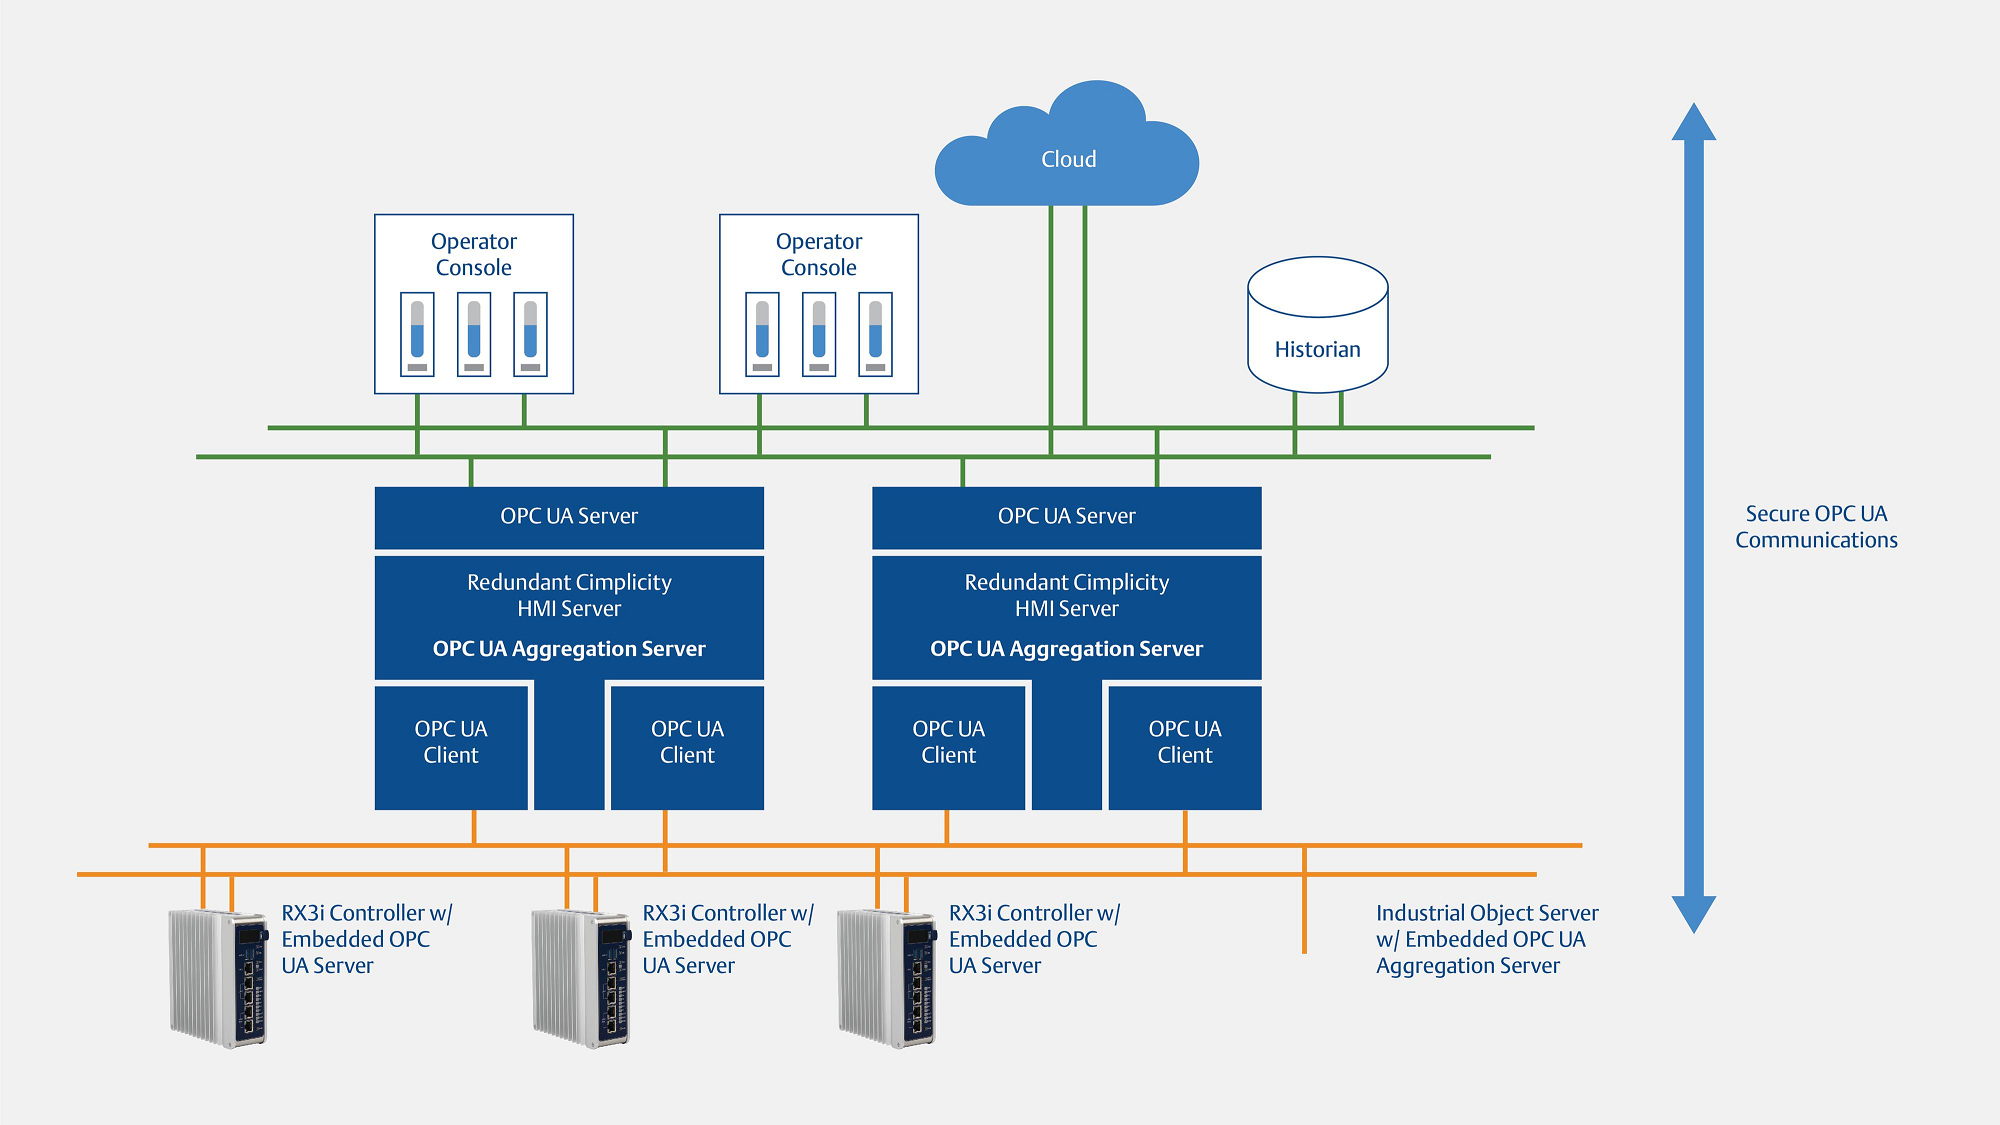
\includegraphics[width=1\textwidth]{figures/Chapter2/opcua.png}
    \caption{Tổng quan OPC UA}
    \label{c2:opcua}
\end{figure}
OPC UA ngày nay không chỉ được triển khai trong PLC, robot và cảm biến mà còn xuất hiện trên các thiết bị nhúng, chip, và thiết bị IoT. Khả năng kết nối chuẩn hóa tạo điều kiện truyền dữ liệu lên các nền tảng đám mây; các tính năng bổ trợ như Cloud Relay giúp vượt qua giới hạn tường lửa. Cùng với sự phát triển của 5G, WiFi 6/7 và các kỹ thuật mạng hỗ trợ QoS, OPC UA hướng tới truyền thông mang tính quyết định (deterministic) cho các ứng dụng công nghiệp thời gian thực.




